\chapter{Consensus Algorithms Exercise 2}

\assignment{
  Consider the electrical network shown in Figure \ref{fig:droop}, where $p_i$ illustrates a droop-controlled inverter.
  \begin{figure}[H]
    \centering
    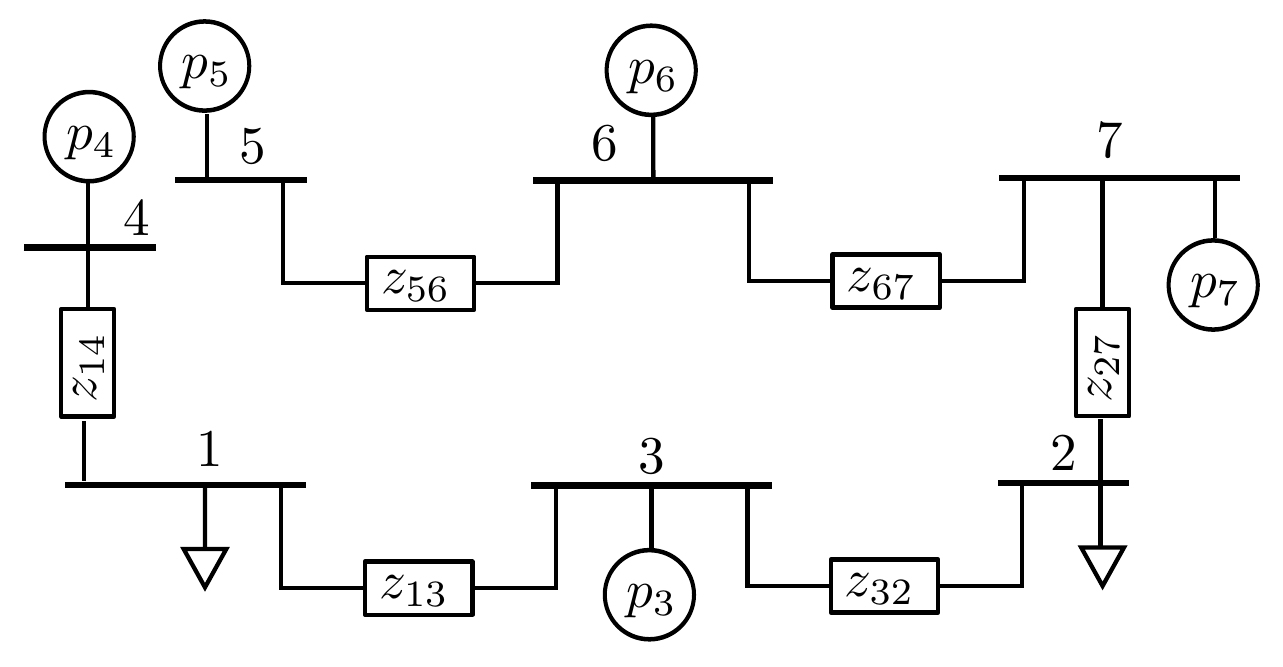
\includegraphics[width=0.7\textwidth]{droop.png}
    \caption{Illustration of an electrical grid.}
    \label{fig:droop}
  \end{figure}
  We assume that the five droop-controlled inverters use the distributed averaging PI control of [Simpson et al., 2013];
  thus, the dynamics of the integral control are
  \begin{equation}
    k_i\dot{p}_i = - \sum_{j\in V_I} L_{c,ij} \left( \frac{p_i}{D_i} - \frac{p_j}{D_j} \right)
  \end{equation}
  In this example $k_i = 10^{-6}$ s for all $i \in V_I$ and $D_i = 4 + (3 - i) \g 0.5$ kWs.
  \begin{itemize}
    \item Design a weighted communication Laplacian such that consensus is reached.
    \item Simulate the system.
    \item How long delay can the system tolerate? (verify your result by simulation)
    \item Change the weighted communication Laplacian such that the system can tolerate twice as long delays.
  \end{itemize}
}
